\documentclass{KPS_assignment}
% ---------For Persian------------
% \newcommand*{\name}{کیوان جمالی}
% \newcommand*{\id}{403209743}
% \newcommand*{\professor}{دکتر شفاهی}
% \newcommand*{\cdate}{2024/12/26}
% \newcommand*{\course}{درس (شماره)}
% \newcommand*{\assignment}{تمرین شماره1}
% ----------For English------------
\newcommand*{\name}{Keivan Jamali}
\newcommand*{\id}{403209743}
\newcommand*{\professor}{Dr. Shafahi}
\newcommand*{\cdate}{1405/03/06}
\newcommand*{\course}{Airport (20\_582)}
\newcommand*{\assignment}{Homework 5}
% ----------START------------------
\usepackage{pgfplots}
\usepackage{float}
\usepackage{amsmath}
\usetikzlibrary{positioning, arrows.meta}
\pgfplotsset{compat=1.18}
\begin{document}
\maketitle
\section*{Problem 1}

There is an airplane with the following properties:

\begin{itemize}
    \item $V$ : airspeed (mile/hr)
    \item $v$ : airspeed (ft/sec)
    \item $\rho_0 = 0.0024 \text{ slugs/ft}^3$ : air density at sea level
    \item $\rho_{36000} = 0.00072 \text{ slugs/ft}^3$ : air density at $36,000 \text{ ft}$
    \item $c = 0.8 \text{ lbs/(lb}\cdot\text{hr)}$ : specific fuel consumption (SFC)
    \item $w_1$ : final weight
    \item $w_0$ : initial weight
    \item $R$ : range (mile) $= \frac{V}{c} \left(\frac{L}{D}\right) \ln\left(\frac{w_0}{w_1}\right) = 2.3 \frac{V}{c} \left(\frac{L}{D}\right) \log_{10}\left(\frac{w_0}{w_1}\right)$
    \item $S = 3000 \text{ ft}^2$ : wing planform area
    \item $S_t = 900 \text{ ft}^2$ : tail planform area
    \item $b = 150 \text{ ft}$ : wingspan
    \item $l = 150 \text{ ft}$ : aircraft length
    \item $d_f = 12 \text{ ft}$ : fuselage diameter
    \item $d_e = 5 \text{ ft}$ : engine diameter
    \item $h$ : altitude in $\text{ft}$
    \item $C''$ : fuel consumption rate ($\text{lb/mile}$)
    \item $a$ : acceleration
    \item $G$ : glide distance
    \item $f = 0.02$ : rolling friction coefficient
    \item $f_b$ : braking friction coefficient
    \item $w_g = 330000 \text{ lbs}$ : gross takeoff weight (GTOW)
    \item $w_e = 150000 \text{ lbs}$ : operating empty weight (OEW)
    \item $w_f = 150000 \text{ lbs}$ : maximum fuel weight
    \item $w_r = 15000 \text{ lbs}$ : reserve fuel weight
    \item $w_p = 100000 \text{ lbs}$ : payload weight ($w_g - w_e - w_f$)
    \item $n = 4$ : number of engines
    \item $T_0 = 4 \times 15000 \text{ lbs}$ : total thrust at sea level
    \item $T_{36000} = 4 \times 4000 \text{ lbs}$ : total thrust at $36,000 \text{ ft}$ altitude
    \item $C_{L_{max}} = 1.5$ : maximum lift coefficient (for landing and takeoff)
    \item $C_D = C_{DP} + C_{DI}$ : total drag coefficient
    \item $C_{DP_{tail}} = 0.01$ : parasite drag coefficient of the tail
    \item $C_{DP_{wing}} = 0.0055$ : parasite drag coefficient of the wing
    \item $C_{DI} = \frac{C_{L}^2}{\pi AR}$ : induced drag coefficient
    \item $AR = \frac{b^2}{S}$ : aspect ratio
    \item $L = C_L \cdot \left(\frac{\rho}{2}\right) \cdot V^2 \cdot S$ : Lift force
    \item $D = C_D \cdot \left(\frac{\rho}{2}\right) \cdot V^2 \cdot S$ : Drag force
\end{itemize}

We want this airplane to move the maximum possible baggage per time from point A to point D. The airplane may stop at B or C for refueling. Each stop (at A, B, C, or D) causes a 1.5‑hour delay. Assume the cruise speed at 36,000 ft is 500 miles per hour.

The available routes and distances (in miles) are shown in Figure 1.

\begin{figure}[H]
\centering
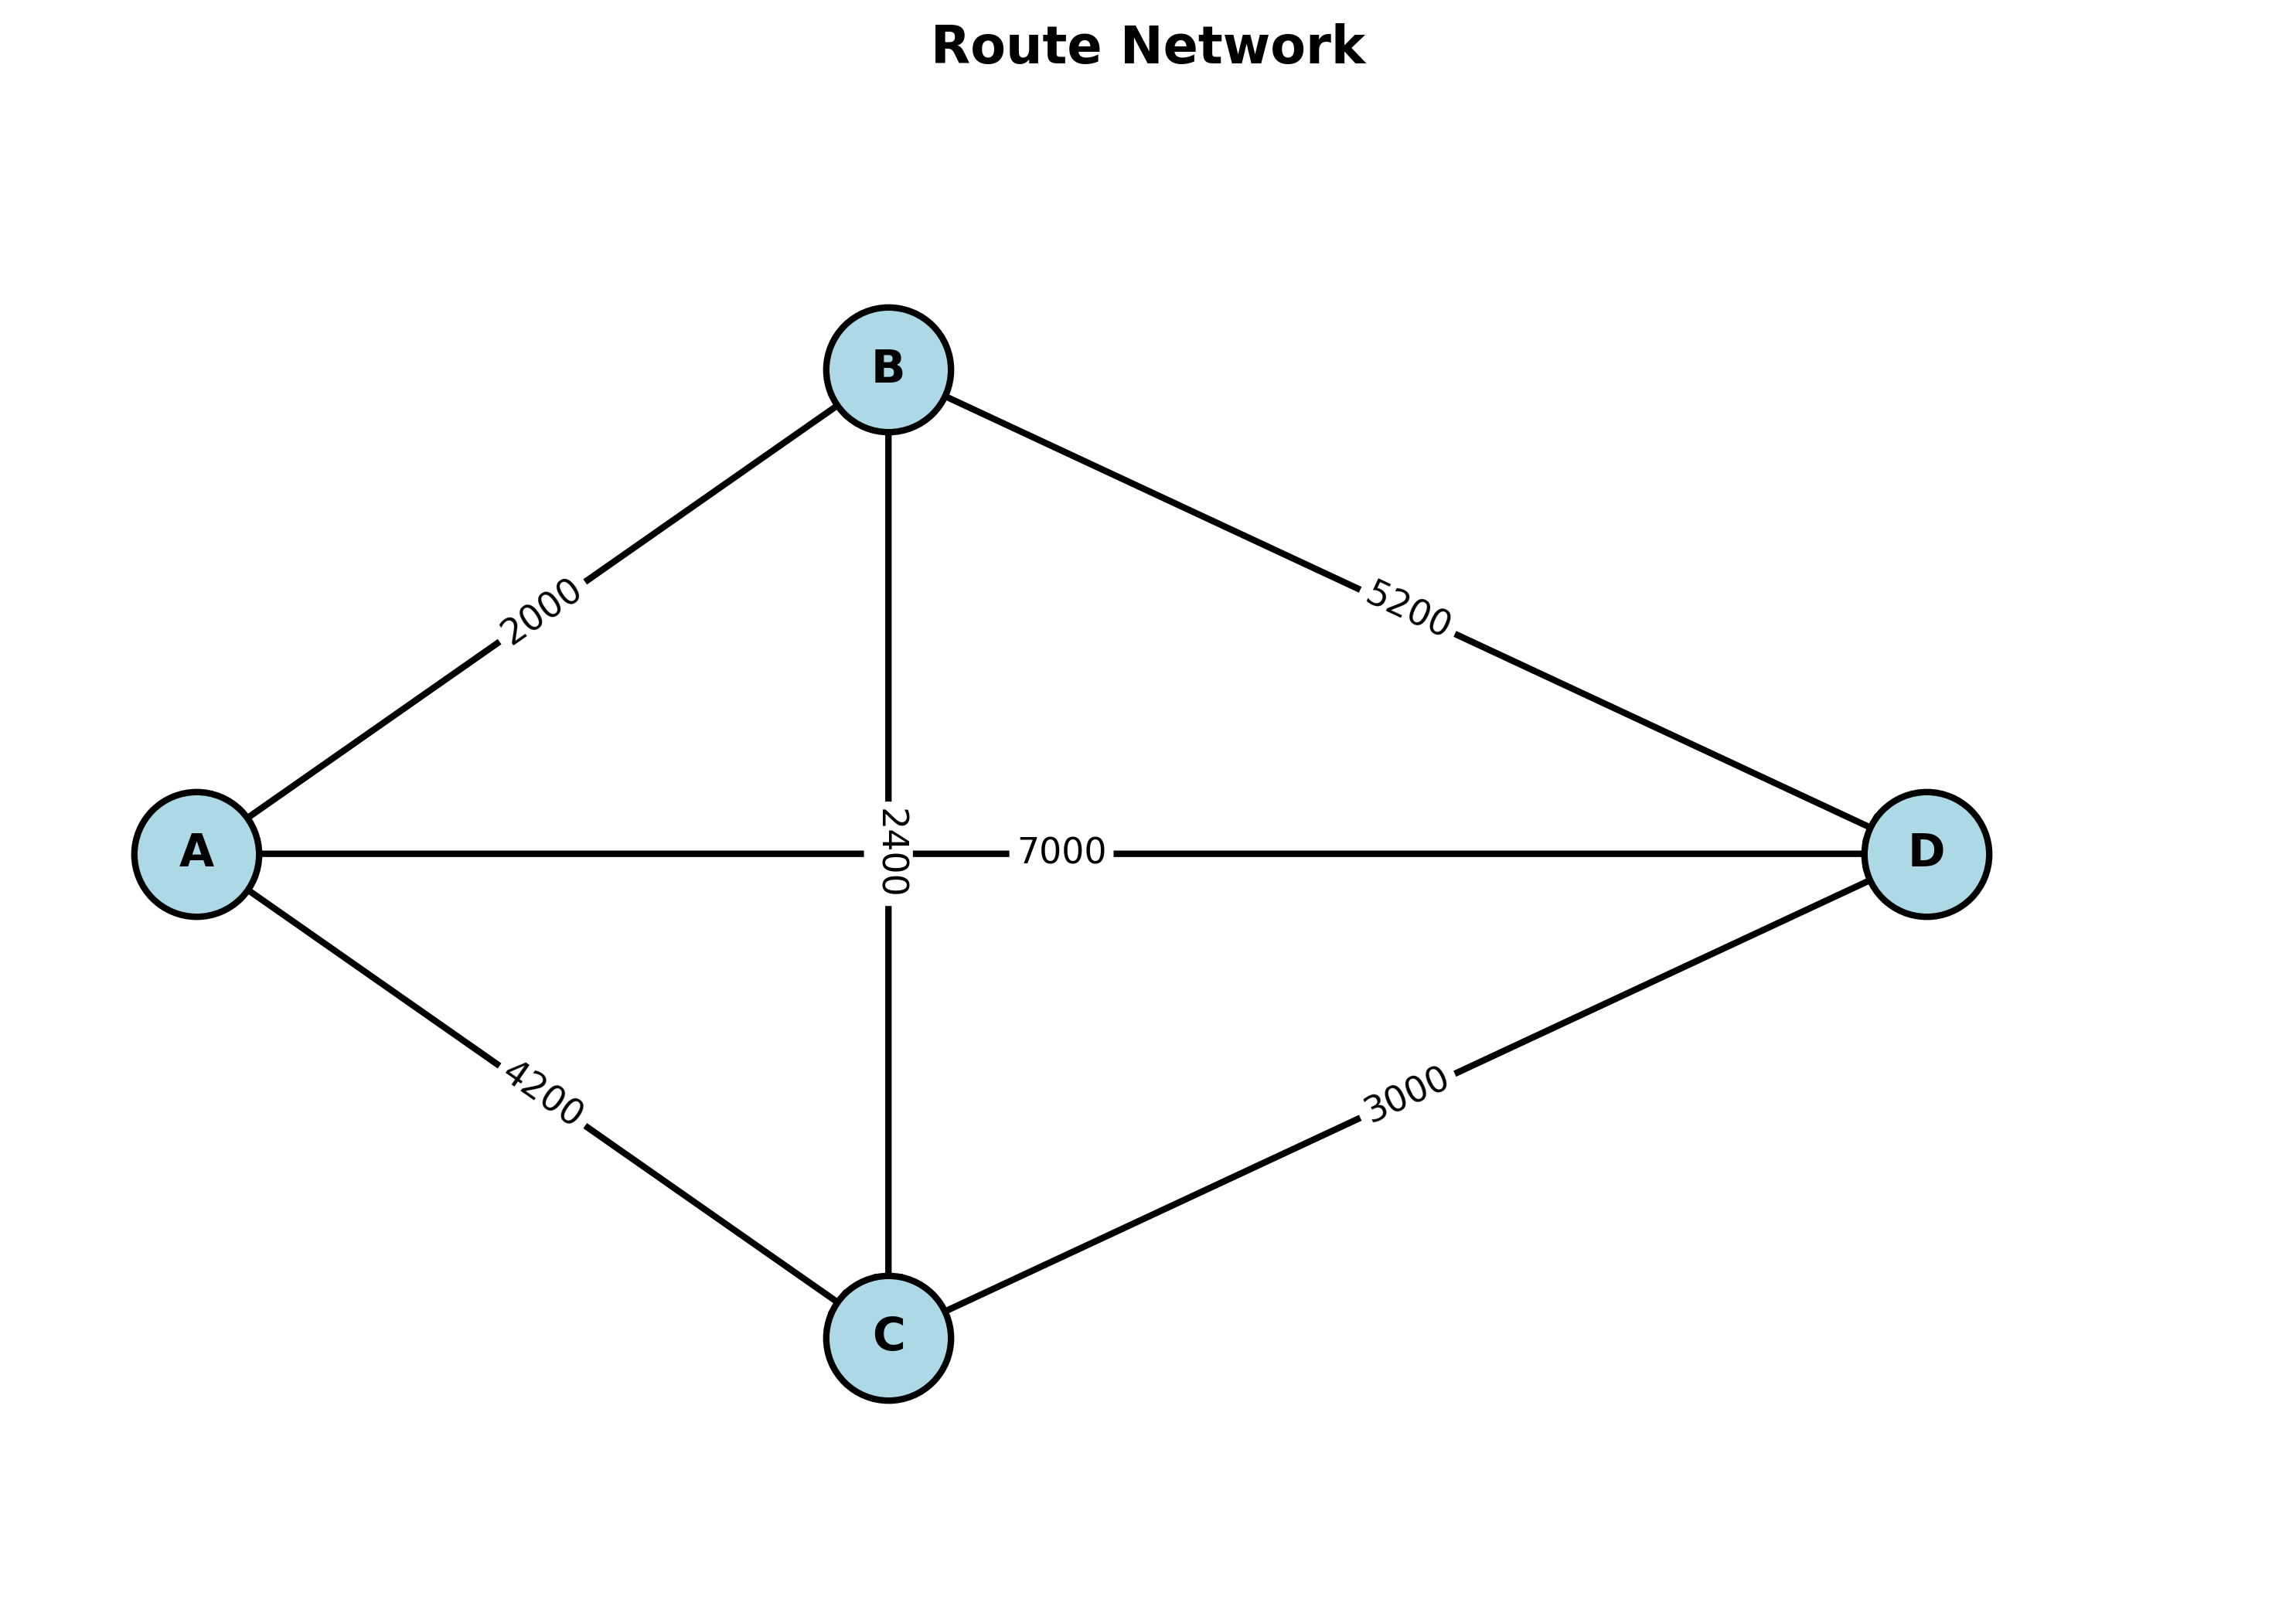
\includegraphics[width=0.7\textwidth]{route_graph.png}
\caption{Route network with distances in miles.}
\label{fig:graph}
\end{figure}

Find:
\begin{enumerate}
    \item Best path (for maximum baggage per day)
    \item Maximum output (pounds per day)
    \item Fuel consumption (pounds of fuel per pound of baggage delivered to D)
    \item For the purpose of better efficiency, redesign the path to minimize fuel consumption (pounds of fuel per ton of baggage delivered to D)
\end{enumerate}

\subsection*{Solution of Problem 1}

\subsubsection{Step 1: Aerodynamic Characteristics}

The aspect ratio of the wing is:

\[
AR=\frac{b^2}{S}
\]

Substituting the given values:

\[
AR=\frac{150^2}{3000}=7.5
\]

The parasite drag coefficient is:

\[
C_{DP}=C_{DP_{tail}}+C_{DP_{wing}}
\]

\[
C_{DP}=0.01+0.0055=0.0155
\]

The induced drag coefficient is:

\[
C_{DI}=\frac{C_L^2}{\pi AR}
\]

The total drag coefficient becomes:

\[
C_D=C_{DP}+C_{DI}
\]

For maximum range, the airplane must operate at maximum aerodynamic efficiency:

\[
\left(\frac{L}{D}\right)_{\max}
=
\frac{1}{2\sqrt{C_{DP}/(\pi AR)}}
\]

Substituting the values:

\[
\left(\frac{L}{D}\right)_{\max}
=
\frac{1}{2\sqrt{0.0155/(\pi\times7.5)}}
\]

\[
\boxed{
\left(\frac{L}{D}\right)_{\max}\approx19.5
}
\]

%------------------------------------------------

\subsubsection{Step 2: Breguet Range Equation}

The aircraft range is given by the Breguet equation:

\[
R=
\frac{V}{c}
\left(\frac{L}{D}\right)
\ln\left(\frac{w_0}{w_1}\right)
\]

where:

\[
V=500 \text{ mile/hr}
\]

\[
c=0.8
\]

\[
\frac{L}{D}=19.5
\]

Define:

\[
K=
\frac{V}{c}
\left(\frac{L}{D}\right)
\]

Thus:

\[
K=
\frac{500}{0.8}\times19.5
\]

\[
\boxed{
K\approx12187.5
}
\]

The maximum takeoff weight is:

\[
w_0=330000 \text{ lb}
\]

The final landing weight is:

\[
w_1=w_e+w_r+P
\]

where \(P\) is the payload.

Since:

\[
w_e=150000 \text{ lb}
\]

\[
w_r=15000 \text{ lb}
\]

then:

\[
w_1=165000+P
\]

Substituting into the Breguet equation:

\[
R=
K
\ln\left(
\frac{330000}{165000+P}
\right)
\]

Solving for payload:

\[
\boxed{
P=
\frac{330000}{e^{R/K}}
-165000
}
\]

This equation gives the maximum payload that can be transported for a given flight distance.

%------------------------------------------------

\subsubsection{Step 3: Maximum Payload for Each Route}

Using the previous equation:

\[
P=
\frac{330000}{e^{R/12187.5}}
-165000
\]

the maximum payload for each route is calculated.

\begin{center}
\begin{tabular}{|c|c|c|}
\hline
Route & Distance (mile) & Maximum Payload (lb) \\
\hline
AB & 2000 & 115043 \\
BC & 2400 & 105998 \\
CD & 3000 & 92976 \\
AC & 4200 & 68779 \\
BD & 5200 & 50358 \\
AD & 7000 & 20781 \\
\hline
\end{tabular}
\end{center}

%------------------------------------------------

\subsubsection{Step 4: Evaluate Possible Paths}

We now calculate the payload throughput for each path.

%------------------------------------------------

\paragraph{Path 1: \(A\rightarrow B\rightarrow C\rightarrow D\)}

The payload is limited by the smallest payload among all legs:

\[
P_{max}=
\min(115043,105998,92976)
\]

\[
\boxed{
P_{max}=92976 \text{ lb}
}
\]

Total flight distance:

\[
R_{total}=2000+2400+3000
\]

\[
R_{total}=7400 \text{ mile}
\]

Flight time:

\[
t_{flight}=
\frac{7400}{500}
=14.8 \text{ hr}
\]

There are four airport operations:

\[
A,B,C,D
\]

Each operation causes a \(1.5\) hr delay:

\[
t_{ground}=4\times1.5=6 \text{ hr}
\]

Total transportation time:

\[
t_{total}=14.8+6
\]

\[
\boxed{
t_{total}=20.8 \text{ hr}
}
\]

Trips per day:

\[
N=
\frac{24}{20.8}
=1.154
\]

Payload transported per day:

\[
Q=
92976\times1.154
\]

\[
\boxed{
Q\approx107000 \text{ lb/day}
}
\]

%------------------------------------------------

\paragraph{Path 2: \(A\rightarrow C\rightarrow D\)}

Payload limitation:

\[
P_{max}=
\min(68779,92976)
\]

\[
P_{max}=68779 \text{ lb}
\]

Total distance:

\[
4200+3000=7200 \text{ mile}
\]

Flight time:

\[
\frac{7200}{500}=14.4 \text{ hr}
\]

Ground delay:

\[
3\times1.5=4.5 \text{ hr}
\]

Total time:

\[
18.9 \text{ hr}
\]

Payload/day:

\[
68779\times\frac{24}{18.9}
\]

\[
\boxed{
Q\approx87300 \text{ lb/day}
}
\]

%------------------------------------------------

\paragraph{Path 3: \(A\rightarrow B\rightarrow D\)}

Payload limitation:

\[
P_{max}=
\min(115043,50358)
\]

\[
P_{max}=50358 \text{ lb}
\]

Total distance:

\[
2000+5200=7200 \text{ mile}
\]

Flight time:

\[
14.4 \text{ hr}
\]

Ground delay:

\[
4.5 \text{ hr}
\]

Total time:

\[
18.9 \text{ hr}
\]

Payload/day:

\[
50358\times\frac{24}{18.9}
\]

\[
\boxed{
Q\approx63900 \text{ lb/day}
}
\]

%------------------------------------------------

\paragraph{Path 4: \(A\rightarrow D\)}

Maximum payload:

\[
P_{max}=20781 \text{ lb}
\]

Flight time:

\[
\frac{7000}{500}=14 \text{ hr}
\]

Ground delay:

\[
2\times1.5=3 \text{ hr}
\]

Total time:

\[
17 \text{ hr}
\]

Payload/day:

\[
20781\times\frac{24}{17}
\]

\[
\boxed{
Q\approx29300 \text{ lb/day}
}
\]

%------------------------------------------------

\paragraph{Step 5: Best Path}

Comparing all paths:

\begin{center}
\begin{tabular}{|c|c|}
\hline
Path & Payload per Day (lb/day) \\
\hline
\(A\rightarrow B\rightarrow C\rightarrow D\) & 107000 \\
\(A\rightarrow C\rightarrow D\) & 87300 \\
\(A\rightarrow B\rightarrow D\) & 63900 \\
\(A\rightarrow D\) & 29300 \\
\hline
\end{tabular}
\end{center}

Therefore, the best path is:

\[
\boxed{
A\rightarrow B\rightarrow C\rightarrow D
}
\]

%------------------------------------------------

\subsubsection{Step 6: Fuel Consumption}

The fuel consumption for one trip is:

\[
w_f=w_0-w_1
\]

For the optimal route:

\[
P=92976 \text{ lb}
\]

Thus:

\[
w_1=165000+92976
\]

\[
w_1=257976 \text{ lb}
\]

The initial weight is:

\[
w_0=330000 \text{ lb}
\]

Therefore:

\[
w_f=330000-257976
\]

\[
\boxed{
w_f=72024 \text{ lb}
}
\]

Fuel consumption per payload pound:

\[
\frac{72024}{92976}
\]

\[
\boxed{
0.775 \text{ lb fuel/lb payload}
}
\]

Fuel consumption per ton of payload:

\[
0.775\times2000
\]

\[
\boxed{
1550 \text{ lb fuel/ton payload}
}
\]

%------------------------------------------------

\subsection{Final Answers}

\begin{enumerate}
    \item Best path:
    \[
    \boxed{
    A\rightarrow B\rightarrow C\rightarrow D
    }
    \]

    \item Maximum payload transportation rate:
    \[
    \boxed{
    1.07\times10^5 \text{ lb/day}
    }
    \]

    \item Fuel consumption:
    \[
    \boxed{
    0.775 \text{ lb fuel/lb payload}
    }
    \]

    \item The most fuel-efficient route is also:
    \[
    \boxed{
    A\rightarrow B\rightarrow C\rightarrow D
    }
    \]


%############################################
%############################################
%############################################
%############################################
\section*{Problem 2}

Determine the minimum runway (or pavement) width required for a Boeing 757-200 aircraft to perform a \(180^\circ\) turn (U-turn).

The following aircraft data are given:

\begin{itemize}
    \item Aircraft length: \(47.3\,\text{m}\)
    \item Wingspan: \(38.1\,\text{m}\)
    \item Wheelbase (distance between nose gear and main landing gear): \(18.29\,\text{m}\)
    \item Maximum nose wheel steering angle (assumed): \(65^\circ\)
\end{itemize}

\subsection*{Answer}

To estimate the required pavement width for a U-turn, the turning radius of the aircraft must first be calculated.

Using the vehicle turning geometry relation:

\[
R = \frac{L}{\tan \theta}
\]

where:

\begin{itemize}
    \item \(R\) = turning radius
    \item \(L = 18.29\,\text{m}\) = wheelbase
    \item \(\theta = 65^\circ\) = maximum steering angle
\end{itemize}

First, calculate:

\[
\tan(65^\circ) \approx 2.145
\]

Therefore:

\[
R = \frac{18.29}{2.145}
\]

\[
R \approx 8.52\,\text{m}
\]

This radius corresponds approximately to the landing gear turning path. However, the aircraft fuselage and wings extend beyond this path, therefore additional swept width must be considered.

For large commercial aircraft, the required pavement width can be approximated as:

\[
W \approx 2R + B
\]

where:

\begin{itemize}
    \item \(W\) = required pavement width
    \item \(R = 8.52\,\text{m}\)
    \item \(B\) = additional swept width caused by fuselage and wing overhang
\end{itemize}

For the Boeing 757-200, the additional swept width is approximately:

\[
B \approx 19.5\,\text{m}
\]

Thus:

\[
W \approx 2(8.52) + 19.5
\]

\[
W \approx 17.04 + 19.5
\]

\[
W \approx 36.5\,\text{m}
\]

Therefore, the minimum pavement width required for a Boeing 757-200 to perform a \(180^\circ\) turn is approximately:

\[
\boxed{W \approx 36.6\,\text{m}}
\]

which is equivalent to:

\[
\boxed{120\,\text{ft}}
\]

It should be noted that this value is also available in Boeing airport planning references and aviation engineering sources, where the published minimum pavement width for a Boeing 757-200 \(180^\circ\) turn is approximately \(36.6\,\text{m}\) (\(120\,\text{ft}\)).


%#############################################
%#############################################
%#############################################
%#############################################
\section*{Problem 3}

The table below presents the profile specifications of a proposed airport runway site. A runway is required for this airport with a \textbf{basic length} of 8000 ft. Apply the following corrections to the runway length:

\begin{itemize}
    \item Add 10\% to the runway length for each 1\% of effective gradient.
    \item Add 7\% to the runway length for every 1000 ft elevation above mean sea level.
\end{itemize}

You are required to design an airport runway at this location in such a way that the FAA regulations are satisfied while minimizing the overall cost. The following cost data are provided:

\begin{itemize}
    \item Pavement cost: \$20 per square foot
    \item Cutting or filling cost: \$0.03 per cubic foot
    \item Borrowing fill material or hauling excess cut material outside the site: \$0.05 per cubic foot
\end{itemize}

Show the ground profile, all calculations, and explain how your design satisfies FAA regulations. (Minor approximations are acceptable.)

\subsection*{Site Profile Data}

\begin{table}[H]
\centering
\begin{tabular}{|c|c|}
\hline
\textbf{Station} & \textbf{Elevation (ft)} \\
\hline
0   & 1020 \\
20  & 980  \\
40  & 980  \\
60  & 1000 \\
80  & 1040 \\
100 & 1020 \\
120 & 990  \\
140 & 1000 \\
160 & 1040 \\
\hline
\end{tabular}
\end{table}


\subsection*{Solution}

The required runway length must first be corrected for both airport elevation and effective gradient according to FAA recommendations.

\subsubsection*{1. Elevation Correction}

The average elevation of the site is calculated from the given profile data:

\[
\bar{E} =
\frac{1020+980+980+1000+1040+1020+990+1000+1040}{9}
\]

\[
\bar{E} =
\frac{9070}{9}
=
1007.8 \text{ ft}
\]

Therefore, the average airport elevation is approximately:

\[
\bar{E} \approx 1008 \text{ ft}
\]

FAA requires a 7\% increase in runway length for every 1000 ft elevation above mean sea level:

\[
\text{Elevation correction}
=
7\% \times \frac{1008}{1000}
=
7.056\%
\]

The corrected runway length becomes:

\[
L_1
=
8000(1+0.07056)
\]

\[
L_1
=
8564.5 \text{ ft}
\]

\subsubsection*{2. Effective Gradient Correction}

The effective gradient is defined as:

\[
G =
\frac{\text{Maximum elevation difference}}{\text{Runway length}}
\times 100
\]

From the profile data:

\[
E_{\max}=1040 \text{ ft}
\]

\[
E_{\min}=980 \text{ ft}
\]

Thus,

\[
\Delta h = 1040-980=60 \text{ ft}
\]

Using the corrected runway length:

\[
G
=
\frac{60}{8564.5}\times100
\]

\[
G \approx 0.70\%
\]

FAA requires a 10\% increase in runway length for each 1\% effective gradient. Therefore:

\[
\text{Gradient correction}
=
0.70 \times 10\%
=
7.0\%
\]

The final corrected runway length becomes:

\[
L_f
=
8564.5(1+0.07)
\]

\[
L_f
=
9163.9 \text{ ft}
\]

Therefore, the required runway length is approximately:

\[
\boxed{9200 \text{ ft}}
\]

\subsubsection*{3. Proposed Runway Profile}

The existing ground profile contains relatively steep changes in elevation, which may violate FAA longitudinal slope recommendations. Therefore, grading operations are required to create a smoother runway profile.

A proposed economical runway profile is shown below:

\begin{table}[h!]
\centering
\begin{tabular}{|c|c|c|c|}
\hline
\textbf{Station} & \textbf{Existing Elevation (ft)} & \textbf{Proposed Elevation (ft)} & \textbf{Cut / Fill (ft)} \\
\hline
0   & 1020 & 1005 & Cut 15 \\
20  & 980  & 1000 & Fill 20 \\
40  & 980  & 1000 & Fill 20 \\
60  & 1000 & 1005 & Fill 5 \\
80  & 1040 & 1010 & Cut 30 \\
100 & 1020 & 1005 & Cut 15 \\
120 & 990  & 1000 & Fill 10 \\
140 & 1000 & 1005 & Fill 5 \\
160 & 1040 & 1010 & Cut 30 \\
\hline
\end{tabular}
\end{table}

This profile smooths the runway grades and reduces abrupt elevation changes, helping satisfy FAA slope limitations.

\subsubsection*{4. Earthwork Evaluation}

Approximate total cut:

\[
15+30+15+30=90
\]

Approximate total fill:

\[
20+20+5+10+5=60
\]

Thus, there is approximately:

\[
90-60=30
\]

units of excess cut material that must be hauled outside the site.

Because the proposed design keeps the cut and fill quantities relatively close, hauling and borrowing costs are minimized.

\subsubsection*{5. Pavement Cost}

Assuming a standard runway width of:

\[
W = 150 \text{ ft}
\]

Runway pavement area:

\[
A = 9200 \times 150
\]

\[
A = 1{,}380{,}000 \text{ ft}^2
\]

Given the pavement cost of \$20 per square foot:

\[
\text{Pavement Cost}
=
1{,}380{,}000 \times 20
\]

\[
=
\$27{,}600{,}000
\]


%#############################################
%#############################################
%#############################################
%#############################################
\section*{Problem 4}

A sketch of the obstruction surfaces defined in FAR Part 77 is shown in Fig. B-1. The obstruction surfaces are to be specified for approaches to a 10,000-ft runway designed for use by transport aircraft for precision-instrument operations. The elevation of the runway is 642.5 ft AMSL.

\begin{enumerate}
    \item[(a)] Determine the coordinates of points A, B, C, D, E, F, and G shown in Fig. B-1.
    
    \item[(b)] Determine whether an object which is 280 ft high located at a point 12,000 ft from the midpoint of the runway along the extended runway centerline penetrates the FAR Part 77 obstruction surfaces.
    
    \item[(c)] Determine the maximum elevation of a tower located at a point 2000 ft from the midpoint of the runway measured along the runway centerline and offset a distance of 8000 ft from the runway centerline, if it is not to penetrate the FAR Part 77 obstruction surfaces.
\end{enumerate}

\subsection*{Answer}

Assume the origin is located at the midpoint of the runway:
\[
(0,0,642.5)
\]
where the \(x\)-axis is along the runway centerline and the \(y\)-axis is perpendicular to the runway.

For a precision-instrument runway according to FAR Part 77:

\begin{itemize}
    \item Horizontal surface elevation:
    \[
    642.5 + 150 = 792.5\ \text{ft}
    \]
    
    \item Conical surface slope:
    \[
    20:1
    \]
    
    \item Approach surface:
    \begin{itemize}
        \item Inner width = \(1000\ \text{ft}\)
        \item Outer width = \(16000\ \text{ft}\)
        \item Length = \(50000\ \text{ft}\)
        \item Slope = \(50:1\) for first \(10000\ \text{ft}\), then \(40:1\)
    \end{itemize}
\end{itemize}

\paragraph{(a) Coordinates of the points}

\[
A=(0,\ 5000,\ 792.5)
\]

\[
B=(0,\ 9000,\ 992.5)
\]

For point \(C\), the approach surface reaches the horizontal surface elevation after:
\[
150 \times 50 = 7500\ \text{ft}
\]
from the start of the approach surface:
\[
x_C = 5200 + 7500 = 12700
\]
The half-width at this point is:
\[
500 + \frac{7500}{50000}\times7500 = 1625
\]
Hence:
\[
C=(12700,\ 1625,\ 792.5)
\]

For point \(G\):
\[
x_G = 5200 + 1000 = 6200
\]
\[
z_G = 642.5 + \frac{1000}{50} = 662.5
\]
\[
y_G = 500 + \frac{7500}{50000}\times1000 = 650
\]
Thus:
\[
G=(6200,\ 650,\ 662.5)
\]

For point \(D\):
\[
x_D = 5200 + 50000 = 55200
\]
Elevation rise:
\[
\frac{10000}{50} + \frac{40000}{40}
=200+1000=1200
\]
Therefore:
\[
D=(55200,\ 0,\ 1842.5)
\]

Point \(E\):
\[
E=(55200,\ 8000,\ 1842.5)
\]

For point \(F\), the transitional surface rises at \(7:1\):
\[
z_F = 1842.5 + \frac{5000}{7} = 2556.8
\]
Hence:
\[
F=(55200,\ 13000,\ 2556.8)
\]

\paragraph{(b) Obstruction check}

The object is located \(12000\ \text{ft}\) from the runway midpoint:

\[
x = 12000
\]

Distance from beginning of approach surface:
\[
12000 - 5200 = 6800\ \text{ft}
\]

Allowed elevation rise:
\[
\frac{6800}{50}=136\ \text{ft}
\]

Maximum permitted elevation:
\[
642.5 + 136 = 778.5\ \text{ft}
\]

Object elevation:
\[
642.5 + 280 = 922.5\ \text{ft}
\]

Since:
\[
922.5 > 778.5
\]

the object penetrates the FAR Part 77 obstruction surface by:
\[
922.5 - 778.5 = 144\ \text{ft}
\]

\paragraph{(c) Maximum tower elevation}

Tower location:
\[
(2000,\ 8000)
\]

Distance from runway center:
\[
r=\sqrt{2000^2+8000^2}=8246\ \text{ft}
\]

Since:
\[
8246 < 10000
\]
the point lies inside the horizontal surface.

Maximum allowable elevation:
\[
792.5\ \text{ft AMSL}
\]

Maximum tower height:
\[
792.5 - 642.5 = 150\ \text{ft}
\]

Therefore, the maximum allowable tower height is:
\[
150\ \text{ft}
\]



%#############################################
%#############################################
%#############################################
%#############################################
\section*{Problem 5}

A rough sizing of the airport site is to be made for an airport with parallel runways to be operated in an IFR environment with arrivals on one runway and departures on the other runway. The thresholds of the runways are not staggered. The airside system is to consist of parallel taxiways serving each runway, the terminal complex on one side of the parallel and the property boundary on the other side. The design aircraft is to be a Boeing 767-200. The terminal is to have parallel concourses perpendicular to the runway centerlines, with nose-in aircraft parking. The top of the concourse will be 28 ft high at the end. The runways are 10,000 ft long.

\begin{enumerate}
    \item[(a)] Determine the separation requirements between runway centerlines, between the runway centerline and a parallel taxiway centerline, between parallel taxiway centerlines, between the runway and the terminal building line, between the runway and the property line, and between concourse faces.
    
    \item[(b)] Determine the area of the apron surface, in acres, between the concourses if six aircraft are parked on each terminal face.
    
    \item[(c)] Determine the property area, in acres, between the property line and the terminal building line from ends of the runways.
    
    \item[(d)] Determine the distance between the runway centerline and the aircraft holding line for takeoffs.
\end{enumerate}

\subsection{Answer}

The design aircraft is the Boeing 767-200, which belongs to Aircraft Design Group V (ADG-V). FAA IFR separation standards for ADG-V aircraft are used.

\paragraph{(a) Separation Requirements}

\begin{itemize}
    \item Runway centerline to runway centerline:
    \[
    \boxed{5000\ \text{ft}}
    \]
    
    \item Runway centerline to parallel taxiway centerline:
    \[
    \boxed{400\ \text{ft}}
    \]
    
    \item Parallel taxiway centerline separation:
    \[
    \boxed{267\ \text{ft}}
    \]
    
    \item Runway centerline to terminal building line:
    \[
    400 + 267 + 160 + 190 = 1017 \approx \boxed{1020\ \text{ft}}
    \]
    
    \item Runway centerline to property line:
    \[
    400 + 267 + 300 = 967 \approx \boxed{1000\ \text{ft}}
    \]
    
    \item Concourse face separation:
    \[
    190 + 250 + 190 = \boxed{630\ \text{ft}}
    \]
\end{itemize}

\paragraph{(b) Apron Area Between Concourses}

Assuming a gate spacing of \(170\ \text{ft}\) per aircraft:

\[
L = 6 \times 170 = 1020\ \text{ft}
\]

Apron width:
\[
W = 630\ \text{ft}
\]

Apron area:
\[
A = 1020 \times 630 = 642600\ \text{ft}^2
\]

Converting to acres:
\[
A = \frac{642600}{43560} \approx \boxed{14.8\ \text{acres}}
\]

\paragraph{(c) Property Area}

Total width between terminal building line and property line:
\[
1020 + 1000 = 2020\ \text{ft}
\]

Runway length:
\[
10000\ \text{ft}
\]

Property area:
\[
A = 2020 \times 10000 = 20.2 \times 10^6\ \text{ft}^2
\]

Converting to acres:
\[
A = \frac{20.2 \times 10^6}{43560}
\approx \boxed{464\ \text{acres}}
\]

\paragraph{(d) Runway Centerline to Holding Position}

For ADG-V precision IFR operations, the holding position distance is:

\[
\boxed{280\ \text{ft}}
\]
\end{document}

